\documentclass[11pt]{article}

\usepackage[a4paper,margin=1in]{geometry}
\usepackage{amsmath,amssymb,amsthm,mathtools}
\usepackage{graphicx}
\usepackage{float}
\usepackage{subcaption}
\usepackage{enumitem}
\usepackage{microtype}
\usepackage{xcolor}
\usepackage{hyperref}
\usepackage{fancyhdr}
\usepackage{lastpage}
\usepackage{tikz}
\usetikzlibrary{arrows.meta,calc,patterns}

\hypersetup{
  colorlinks=true,
  linkcolor=blue,
  urlcolor=blue,
  citecolor=blue
}

\setlist[enumerate]{itemsep=0.25em,topsep=0.25em}
\setlength{\parindent}{0pt}
\setlength{\parskip}{0.5em}

\theoremstyle{definition}
\newtheorem{exercise}{Exercise}[section]

\newenvironment{solution}{\begin{proof}[Solution]}{\end{proof}}

\DeclareMathOperator{\Area}{Area}
\DeclareMathOperator{\Vol}{Vol}

\pagestyle{fancy}
\fancyhf{}
\setlength{\headheight}{18.1pt}
\renewcommand{\headrulewidth}{0.4pt}
\fancyhead[L]{\IfFileExists{hkust-crest.png}{
\includegraphics[height=14pt]{hkust-crest.png}}{}}
\fancyhead[C]{MATH1014 Calculus II Tutorial}
\fancyhead[R]{Week 2}
\fancyfoot[C]{\thepage\ /\ \pageref{LastPage}}

\title{\vspace{-1.0em}MATH1014 Calculus II Tutorial\\Week 2}
\author{Wenkai Fan}
\date{}

\begin{document}
\maketitle
\thispagestyle{fancy}

\section{Review}

\subsection{Fundamental Theorem of Calculus (FTC)}
\begin{enumerate}
  \item If $F'(x)=f(x)$ on an interval, then
  \[
  \int_a^b f(t)\,dt=F(b)-F(a).
  \]
  \item If $f$ is continuous and $A(x)=\int_a^x f(t)\,dt$, then
  \[
  A'(x)=f(x).
  \]
  \item Indefinite integrals: $\displaystyle \int f(x)\,dx=F(x)+C$ where $F'(x)=f(x)$.
\end{enumerate}

\subsection{Area Between Curves}
\begin{enumerate}
  \item Using $dx$ (vertical slices): if $y=f(x)$ is above $y=g(x)$ on $[a,b]$, then
  \[
  \Area=\int_a^b \bigl(f(x)-g(x)\bigr)\,dx.
  \]
  \item Using $dy$ (horizontal slices): if $x=h(y)$ is right of $x=k(y)$ on $[c,d]$, then
  \[
  \Area=\int_c^d \bigl(h(y)-k(y)\bigr)\,dy.
  \]
  \item If the top/bottom (or right/left) changes, split the interval at intersection points.
\end{enumerate}

\subsection{Volumes}
\begin{enumerate}
  \item Slicing (cross-sectional area): if the slice area is $A(x)$ for $x\in[a,b]$, then
  \[
  \Vol=\int_a^b A(x)\,dx.
  \]
  \item Cylindrical shells: rotating a vertical strip about the $y$-axis,
  \[
  \Vol=\int_a^b 2\pi\,r(x)\,h(x)\,dx.
  \]
\end{enumerate}

% \begin{figure}[H]
%   \centering
%   \begin{subfigure}[t]{0.32\textwidth}
%     \centering
%     \begin{tikzpicture}[scale=0.9,>=Latex]
%       \draw[->] (0,0) -- (4.2,0) node[below] {$t$};
%       \draw[->] (0,0) -- (0,3.2) node[left] {$y$};
%       \draw[thick,blue] (0.5,0.6) .. controls (1.5,2.6) and (2.7,0.9) .. (3.8,2.4);
%       \fill[blue!20] (1.2,0) -- (1.2,1.55)
%         .. controls (1.7,2.55) and (2.4,1.1) .. (3.2,1.7)
%         -- (3.2,0) -- cycle;
%       \draw (1.2,0) node[below] {$a$};
%       \draw (3.2,0) node[below] {$x$};
%       \draw[dashed] (1.2,0) -- (1.2,1.55);
%       \draw[dashed] (3.2,0) -- (3.2,1.7);
%       \node at (2.2,2.85) {$\int_a^x f(t)\,dt$};
%     \end{tikzpicture}
%     \caption*{FTC: area function}
%   \end{subfigure}\hfill
%   \begin{subfigure}[t]{0.32\textwidth}
%     \centering
%     \begin{tikzpicture}[scale=0.9,>=Latex]
%       \draw[->] (0,0) -- (4.2,0) node[below] {$x$};
%       \draw[->] (0,0) -- (0,3.2) node[left] {$y$};
%       \draw[thick,blue] (0.4,2.4) .. controls (1.4,3.0) and (2.4,1.5) .. (3.8,2.5) node[right] {$f$};
%       \draw[thick,red] (0.4,1.0) .. controls (1.5,1.6) and (2.6,0.6) .. (3.8,1.2) node[right] {$g$};
%       \fill[gray!20] (1.0,0) -- (1.0,1.15)
%         .. controls (1.6,1.55) and (2.4,0.8) .. (3.2,1.1)
%         -- (3.2,2.25)
%         .. controls (2.2,1.45) and (1.6,2.8) .. (1.0,2.55)
%         -- cycle;
%       \draw (1.0,0) node[below] {$a$};
%       \draw (3.2,0) node[below] {$b$};
%       \draw[dashed] (1.0,0) -- (1.0,2.55);
%       \draw[dashed] (3.2,0) -- (3.2,2.25);
%       \node at (2.1,2.95) {$\int_a^b (f-g)\,dx$};
%     \end{tikzpicture}
%     \caption*{Area between curves}
%   \end{subfigure}\hfill
%   \begin{subfigure}[t]{0.32\textwidth}
%     \centering
%     \begin{tikzpicture}[scale=0.9,>=Latex]
%       \draw[->] (0,0) -- (4.2,0) node[below] {$x$};
%       \draw[->] (0,0) -- (0,3.2) node[left] {$A(x)$};
%       \draw[thick,teal!70!black] (0.4,0.6) .. controls (1.2,2.5) and (2.4,0.7) .. (3.8,2.4);
%       \fill[teal!20] (1.0,0) -- (1.0,1.55)
%         .. controls (1.6,2.65) and (2.5,0.95) .. (3.2,1.95)
%         -- (3.2,0) -- cycle;
%       \draw (1.0,0) node[below] {$a$};
%       \draw (3.2,0) node[below] {$b$};
%       \draw[dashed] (1.0,0) -- (1.0,1.55);
%       \draw[dashed] (3.2,0) -- (3.2,1.95);
%       \node at (2.1,2.95) {$V=\int_a^b A(x)\,dx$};
%     \end{tikzpicture}
%     \caption*{Slicing idea}
%   \end{subfigure}
% \end{figure}

% \begin{figure}[H]
%   \centering
%   \begin{tikzpicture}[scale=1.0,>=Latex]
%     \draw[->] (-0.2,0) -- (5.2,0) node[below] {$x$};
%     \draw[->] (0,-0.2) -- (0,3.8) node[left] {$y$};
%     \draw[thick,blue] (0.3,0.2) .. controls (1.2,3.0) and (3.3,3.2) .. (4.8,1.0) node[right] {$y=f(x)$};
%     \draw[thick] (0.3,0.2) -- (4.8,0.2) node[right] {$y=g(x)$};
%     \fill[gray!20] (2.7,0.2) rectangle (2.95,2.55);
%     \draw[<->] (0,0.05) -- (2.83,0.05) node[midway,below] {$r(x)=x$};
%     \draw[<->] (3.05,0.2) -- (3.05,2.55) node[midway,right] {$h(x)=f(x)-g(x)$};
%     \node at (3.6,3.35) {$V=\int_a^b 2\pi r(x)h(x)\,dx$};
%   \end{tikzpicture}
%   \caption*{Cylindrical shells (about the $y$-axis): radius $\times$ height $\times$ thickness}
% \end{figure}

\section{Exercises}

\begin{exercise}[Warm-up: identifying ``top'' and ``bottom'']
Evaluate the area of the following regions enclosed by the given curves.
\begin{enumerate}
  \item $y=\frac{1}{x}$, $y=x$, $x=2$.
  \item $y^2=4(x+1)$, $y^2=4(1-x)$.
  \item $y=\cos x$, $y=\sin 2x$, $x=0$, $x=\frac{\pi}{2}$.
\end{enumerate}
\end{exercise}

\begin{solution}
\textbf{Idea.} For area between curves using $dx$, we aim for
\[
\Area=\int_{x=\text{left}}^{x=\text{right}} \bigl(y_{\text{top}}(x)-y_{\text{bottom}}(x)\bigr)\,dx,
\]
and we split the interval whenever the identity of the top/bottom curve changes.

\textbf{(1)} The curves $y=x$ and $y=\frac{1}{x}$ intersect at $x=1$ (with $y=1$). On $[1,2]$, the line is above the hyperbola, so
\[
\Area=\int_{1}^{2}\left(x-\frac{1}{x}\right)\,dx
=\left.\left(\frac{x^{2}}{2}-\ln x\right)\right|_{1}^{2}
=\frac{3}{2}-\ln 2.
\]

\textbf{(2)} Rewrite each parabola as $x$ in terms of $y$:
\[
y^2=4(x+1)\Rightarrow x=\frac{y^2}{4}-1,\qquad
y^2=4(1-x)\Rightarrow x=1-\frac{y^2}{4}.
\]
It is symmetric about the $x$-axis, so compute the upper half ($y\ge 0$) and double:
\[
\Area=2\int_{0}^{2}\left[\left(1-\frac{y^{2}}{4}\right)-\left(\frac{y^{2}}{4}-1\right)\right]dy
=2\int_{0}^{2}\left(2-\frac{y^{2}}{2}\right)dy
=\frac{16}{3}.
\]

\textbf{(3)} First find intersection points. Solve $\cos x=\sin 2x=2\sin x\cos x$.
Either $\cos x=0$ giving $x=\frac{\pi}{2}$, or $1=2\sin x$ giving $x=\frac{\pi}{6}$ (within $[0,\frac{\pi}{2}]$).
On $[0,\frac{\pi}{6}]$, $\cos x\ge \sin 2x$; on $[\frac{\pi}{6},\frac{\pi}{2}]$, $\sin 2x\ge \cos x$. Hence
\[
\Area=\int_{0}^{\frac{\pi}{6}}(\cos x-\sin 2x)\,dx+\int_{\frac{\pi}{6}}^{\frac{\pi}{2}}(\sin 2x-\cos x)\,dx
=\frac{1}{2}.
\]
\textbf{Checkpoint.} An equivalent one-line setup is $\Area=\int_{0}^{\frac{\pi}{2}}\lvert \cos x-\sin 2x\rvert\,dx$.

\IfFileExists{1_1.jpeg}{
\begin{figure}[H]
  \centering
  \begin{minipage}[t]{0.47\textwidth}
    \centering
    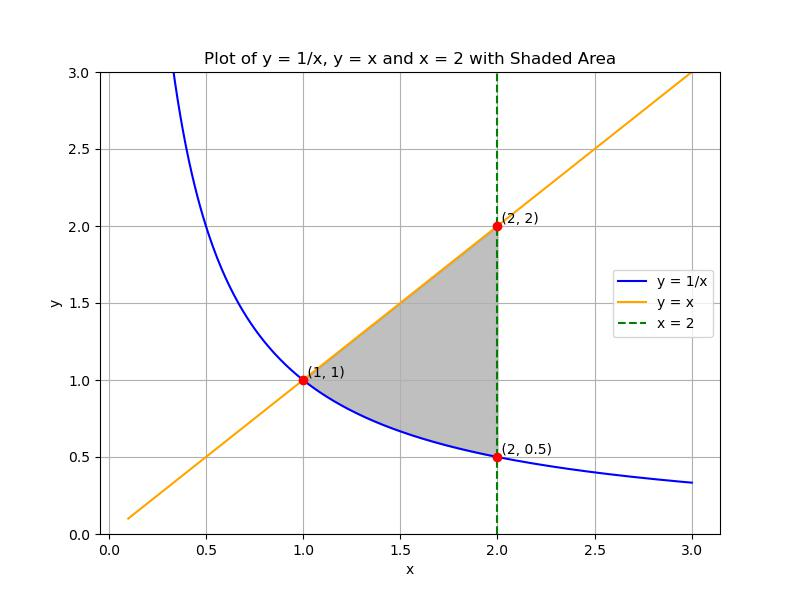
\includegraphics[width=\textwidth]{1_1}
    \caption*{Sketch for (1).}
  \end{minipage}\hfill
  \begin{minipage}[t]{0.47\textwidth}
    \centering
    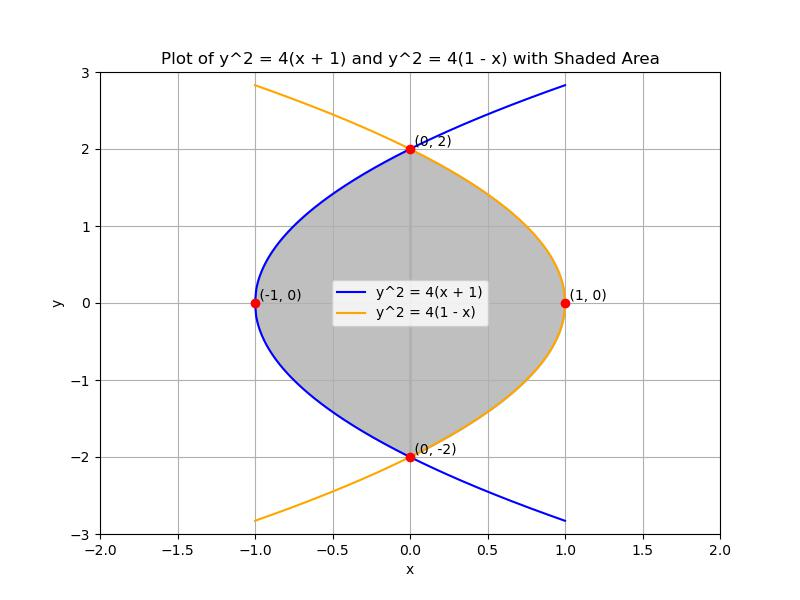
\includegraphics[width=\textwidth]{1_2}
    \caption*{Sketch for (2).}
  \end{minipage}
\end{figure}
}{}

\IfFileExists{1_3.jpeg}{
\begin{figure}[H]
  \centering
  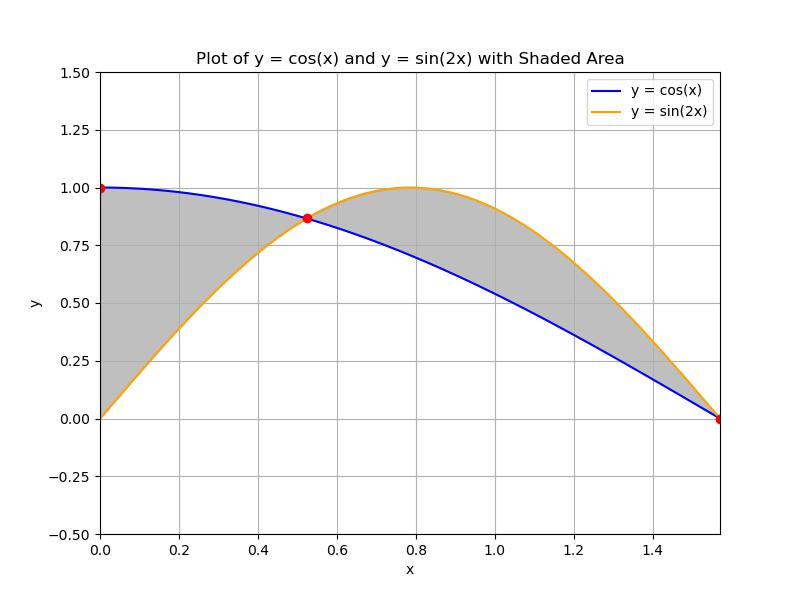
\includegraphics[width=0.6\textwidth]{1_3}
  \caption*{Sketch for (3).}
\end{figure}
}{}

\end{solution}

\begin{exercise}[Area with parameters / splitting regions]
Consider the region enclosed by $y=\frac{1}{x^2}$, $y=-\frac{4}{x^3}$, $x=1$, $x=4$.
\begin{enumerate}
  \item Evaluate the area of the region.
  \item Find a line $x=a$ such that the area of the left part divided by this line equals $2$.
  \item Find a line $y=b$ such that the ratio of area for the upper part and that for the lower part is $1:6$.
\end{enumerate}
\end{exercise}

\begin{solution}
\textbf{Idea.} On $[1,4]$, we have $\frac{1}{x^{2}}>0$ and $-\frac{4}{x^{3}}<0$, so the total area is the integral of (top minus bottom).

\textbf{(1)}\,
\[
\Area=\int_{1}^{4}\left(\frac{1}{x^{2}}-\left(-\frac{4}{x^{3}}\right)\right)dx
=\int_{1}^{4}\left(\frac{1}{x^{2}}+\frac{4}{x^{3}}\right)dx
=\left.-\frac{1}{x}-\frac{2}{x^{2}}\right|_{1}^{4}
=\frac{21}{8}.
\]

\textbf{(2)} Let $A(a)=\int_{1}^{a}\left(\frac{1}{x^{2}}+\frac{4}{x^{3}}\right)dx$. Solve $A(a)=2$:
\[
\left.-\frac{1}{x}-\frac{2}{x^{2}}\right|_{1}^{a}=2
\;\Rightarrow\;
-\frac{1}{a}-\frac{2}{a^{2}}+3=2
\;\Rightarrow\;
a^{2}-a-2=0.
\]
So $a=2$ or $a=-1$; the interval condition $1<a<4$ forces $a=2$.

\textbf{(3)} Split into the part above the $x$-axis and below the $x$-axis.
Upper area:
\[
A_{\text{upper}}=\int_{1}^{4}\frac{1}{x^{2}}dx=\left.-\frac{1}{x}\right|_{1}^{4}=\frac{3}{4}.
\]
Lower area:
\[
A_{\text{lower}}=\Area-A_{\text{upper}}=\frac{21}{8}-\frac{3}{4}=\frac{15}{8}.
\]
The line $y=b$ splits the whole region into an \emph{upper part} (above $y=b$) and a \emph{lower part} (below $y=b$). The required ratio is
\[
\Area_{\text{above }y=b}:\Area_{\text{below }y=b}=1:6,
\]
so the upper part has area $\Area_{\text{above }y=b}=\frac{1}{7}\Area=\frac{1}{7}\cdot\frac{21}{8}=\frac{3}{8}$.

Because $\frac{3}{8}<A_{\text{upper}}=\frac{3}{4}$, the cutting line must lie above the $x$-axis, so $0<b<1$.
Express the upper curve as $x=\frac{1}{\sqrt{y}}$ (from $y=\frac{1}{x^{2}}$) and the right boundary as $x=1$ at the left end of the region in $xy$-plane for $y\in[b,1]$. Hence the area above $y=b$ in the upper region is
\[
\int_{b}^{1}\left(\frac{1}{\sqrt{y}}-1\right)\,dy
=\left.(2\sqrt{y}-y)\right|_{b}^{1}
=1-2\sqrt{b}+b.
\]
Set it equal to $\frac{3}{8}$:
\[
1-2\sqrt{b}+b=\frac{3}{8}
\;\Rightarrow\;
(\sqrt{b}-1)^{2}=\frac{3}{8}
\;\Rightarrow\;
\sqrt{b}=1-\frac{\sqrt{6}}{4},
\]
so
\[
b=\left(1-\frac{\sqrt{6}}{4}\right)^{2}=\frac{11-4\sqrt{6}}{8}.
\]

\IfFileExists{2.jpeg}{
\begin{figure}[H]
  \centering
  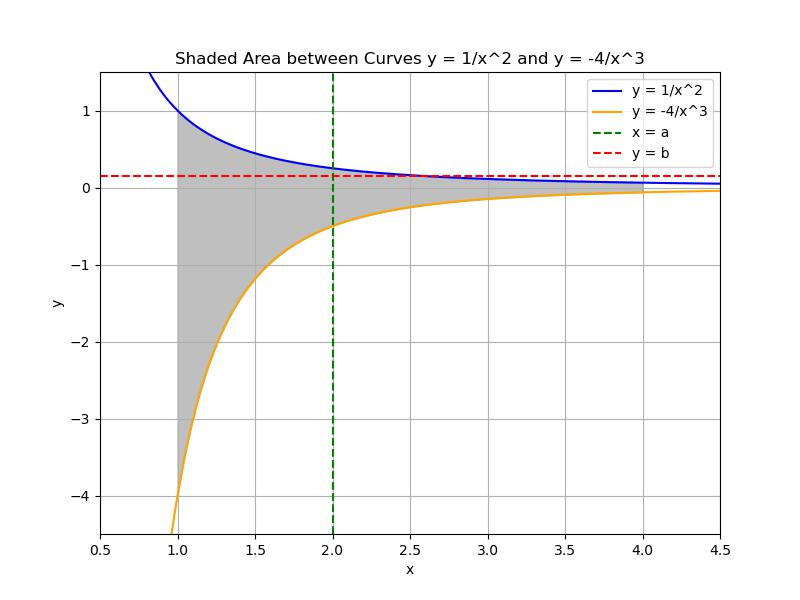
\includegraphics[width=0.65\textwidth]{2}
  \caption*{Sketch for Exercise 2.}
\end{figure}
}{}

\end{solution}

\begin{exercise}[Slicing method]
Evaluate the following volumes.
\begin{enumerate}
  \item An elliptical frustum: the upper base is an ellipse with semi-axes $a,b$. The lower base is an ellipse with semi-axes $A,B$. The height is $h$.
  \item An ellipsoid: $\frac{x^2}{a^2}+\frac{y^2}{b^2}+\frac{z^2}{c^2}\le 1$.
\end{enumerate}
\end{exercise}

\begin{solution}
\textbf{Idea.} For solids with ``nice'' cross-sections, write volume as
\[
\Vol=\int (\text{area of slice})\,d(\text{height}).
\]

\textbf{(1)} Slice the frustum by planes parallel to the bases. At height $x$ from the \emph{top} base (so $x=0$ at the top, $x=h$ at the bottom), the semi-axes change linearly:
\[
a(x)=a+\frac{A-a}{h}x,\qquad b(x)=b+\frac{B-b}{h}x.
\]
So the slice area is $\pi a(x)b(x)$ and
\begin{align*}
\Vol
&=\int_{0}^{h}\pi\left(a+\frac{A-a}{h}x\right)\left(b+\frac{B-b}{h}x\right)\,dx \\
&=\frac{\pi h}{6}\left(2AB+2ab+Ab+aB\right).
\end{align*}

\textbf{(2)} For a fixed $z$ (with $-c\le z\le c$), the cross-section is the ellipse
\[
\frac{x^{2}}{a^{2}}+\frac{y^{2}}{b^{2}}=1-\frac{z^{2}}{c^{2}},
\]
whose semi-axes are $a\sqrt{1-\frac{z^{2}}{c^{2}}}$ and $b\sqrt{1-\frac{z^{2}}{c^{2}}}$. Therefore the slice area is
\[
\pi ab\left(1-\frac{z^{2}}{c^{2}}\right),
\]
and
\[
\Vol=\int_{-c}^{c}\pi ab\left(1-\frac{z^{2}}{c^{2}}\right)dz=\frac{4}{3}\pi abc.
\]

\IfFileExists{3_1_v.png}{
\begin{figure}[H]
  \centering
  \begin{minipage}[t]{0.47\textwidth}
    \centering
    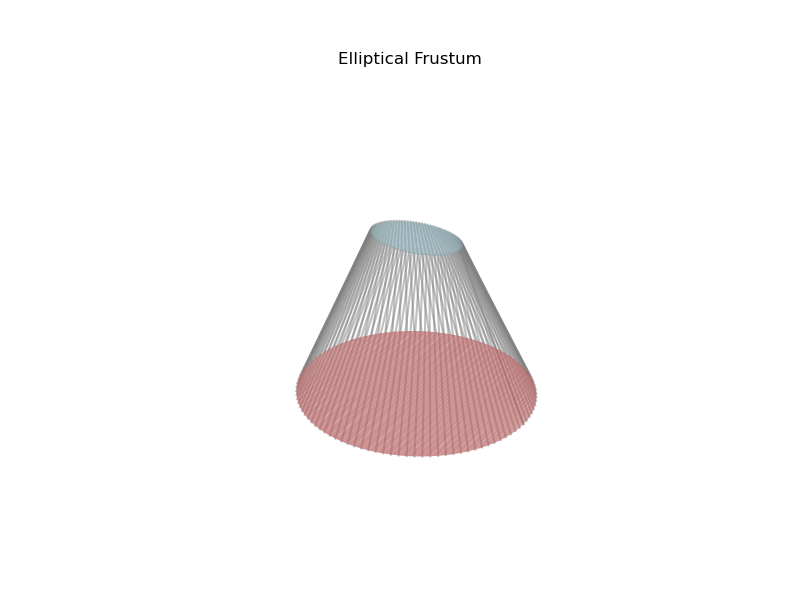
\includegraphics[width=\textwidth]{3_1_v}
    \caption*{Elliptical frustum.}
  \end{minipage}\hfill
  \begin{minipage}[t]{0.47\textwidth}
    \centering
    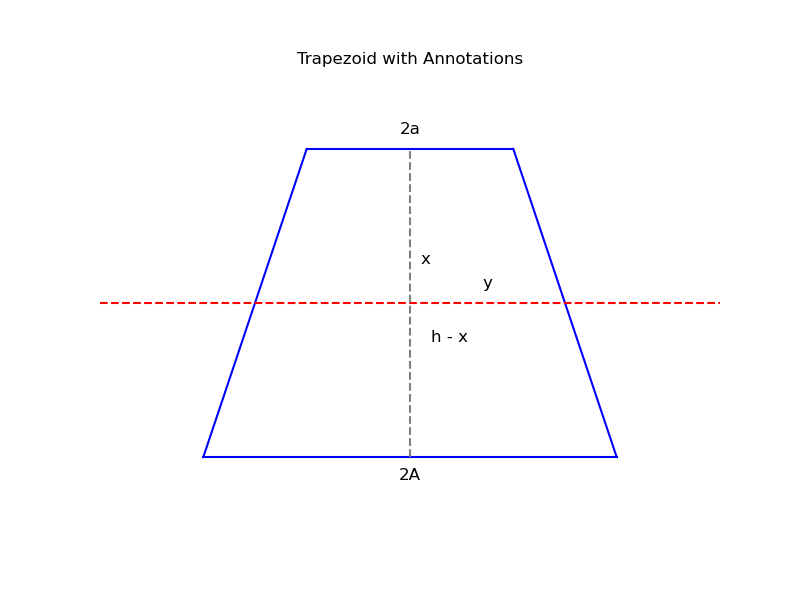
\includegraphics[width=\textwidth]{3_1_a}
    \caption*{Vertical section view.}
  \end{minipage}
\end{figure}
}{}

\IfFileExists{3_2.png}{
\begin{figure}[H]
  \centering
  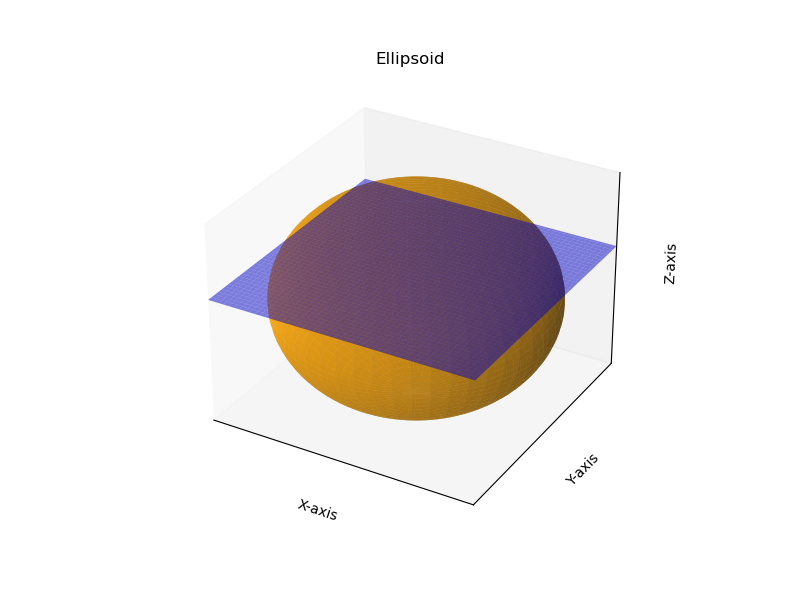
\includegraphics[width=0.62\textwidth]{3_2}
  \caption*{Ellipsoid slicing.}
\end{figure}
}{}

\end{solution}

\begin{exercise}[Washer method and symmetry]
Find the relationship between $a$ and $c$ such that the volumes generated by rotating the arc segment bounded by $y=x(x-a)$ and $y=0$ around the $x$-axis within the intervals $[0,a]$ and $[a,c]$ are equal.
\end{exercise}

\begin{solution}
\textbf{Idea.} Rotating $y=f(x)$ around the $x$-axis gives a volume element $\pi (f(x))^{2}\,dx$ (disk method). Because the radius is squared, the sign of $f(x)$ does not matter.

On $[0,a]$, the function $x(x-a)\le 0$; on $[a,c]$, $x(x-a)\ge 0$. In both cases, the radius squared is $[x(x-a)]^{2}$.

So the volumes are
\[
V_{1}=\int_{0}^{a}\pi[x(x-a)]^{2}\,dx,\qquad
V_{2}=\int_{a}^{c}\pi[x(x-a)]^{2}\,dx.
\]
Compute an antiderivative:
\[
\int \pi[x(x-a)]^{2}\,dx
=\pi\left(\frac{x^{5}}{5}-\frac{a x^{4}}{2}+\frac{a^{2}x^{3}}{3}\right).
\]
Thus
\[
V_{1}=\pi\left(\frac{a^{5}}{5}-\frac{a\cdot a^{4}}{2}+\frac{a^{2}\cdot a^{3}}{3}\right)=\pi\cdot\frac{a^{5}}{30},
\]
and
\[
V_{2}=\pi\left(\frac{c^{5}}{5}-\frac{a c^{4}}{2}+\frac{a^{2}c^{3}}{3}\right)-\pi\cdot\frac{a^{5}}{30}.
\]
Setting $V_{1}=V_{2}$ and cancelling $\pi$ gives the relationship
\[
2a^{5}+15ac^{4}-10a^{2}c^{3}-6c^{5}=0.
\]

\IfFileExists{4.png}{
\begin{figure}[H]
  \centering
  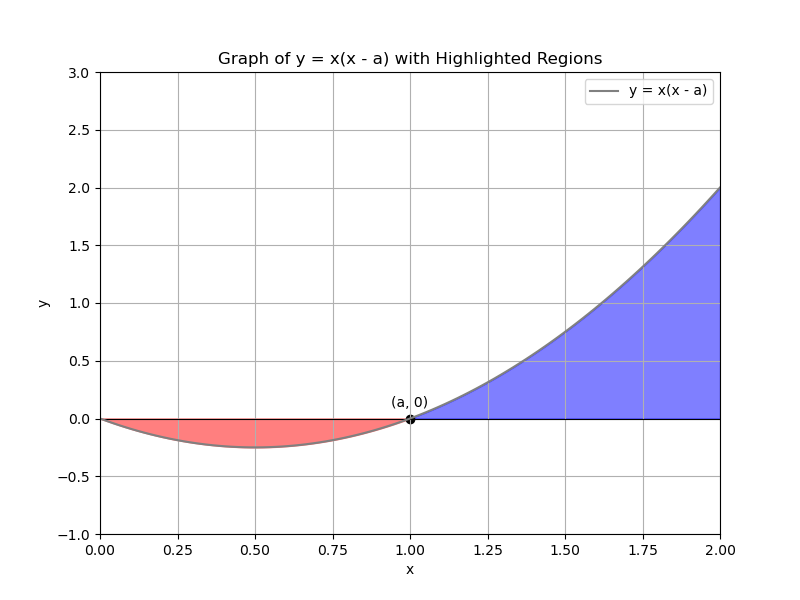
\includegraphics[width=0.6\textwidth]{4}
  \caption*{Sketch for Exercise 4.}
\end{figure}
}{}

\end{solution}

\end{document}
